\section{Model}
\subsection{Flow graph - Overview}

In this work, we consider a number of vessels that each sail with cargo between ports in two regions within a given time frame.  
The vessels' journeys can be illustrated in a network of \emph{port calls} as in Figure~\ref{fig:timespace}, where the horizontal axis illustrates time (the ordered set of \emph{dates}, $\mc{D}$, where port calls happens), while the vertical axis is made up by the set of \emph{ports} ($\mc{P}$). At a port call, cargo can be loaded to the vessel from the yard, or cargo can be discharged from the vessel to the yard. On the other hand, cargo at the yard of a port $p$ can be left at the yard until the next port call at $p$, as the dashed lines in Figure~\ref{fig:timespace} indicates. 

\begin{figure}[htbp]
	\centering
		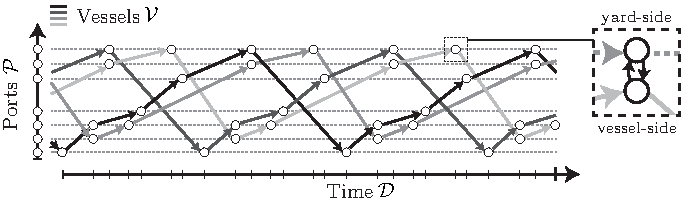
\includegraphics[scale = 1.3]{netwBW.pdf}
		\caption{A network of port calls showing four vessels sailing on routes between seven ports in two different regions. One of the port calls has been magnified to show part of the resulting flow graph.}  \label{fig:timespace}
\end{figure}

At each port call, containers can be exported from land, that is, it can be introduced to the yard at a port call, where it will eventually be picked up by a vessel. It is then transported through the network until it reaches its destination, where it is imported to land. At any port call on its way, it can be transshipped as described above. 
The fist date in the network corresponds to the current state of the network, and hence there is already cargo on the vessels and possibly cargo at the yards of the ports.  

In this way, the network of port calls in Figure~\ref{fig:timespace} only gives a birds eye view of the flow graph $(\mc{N},\mc{E})$ that our model will be based on. In the detailed flow graph, each port call corresponds to a \emph{yard-side} node (in the set $\mc{N}^\ttt{y}\subset \mc{N}$) and a \emph{vessel-side} node (in the set $\mc{N}^\ttt{v}\subset\mc{N}$). In Figure~\ref{fig:timespace}, one of the port calls has been enlarged to show the corresponding vessel-side node and port-side node in this flow graph. The edges between the yard-side node and the vessel-side node correspond to loading and discharging of cargo between the vessel and the yard. The nodes $\mc{N}^\ttt{y}$ and $\mc{N}^\ttt{v}$ makes up the nodes of the flow network that are neither sources nor sinks. %Each of these nodes therefore has a port, a date, and a vessel associated with them.
Besides these nodes, $\mc{N}$ is comprised of the sources $I^\ttt{x}$, $I^\ttt{p}$, and $I^\ttt{v}$, denoting a common export node, a common source for the cargo at yards, and a common source for the cargo aboard the vessel, plus the sinks $O^\ttt{x}$, $O^\ttt{p}$, and $O^\ttt{v}$, which likewise are a common sink for import of cargo, cargo at yards after the last date within the time frame, and cargo on the vessel after the last date, respectively. Note that in Figure~\ref{fig:timespace}, edges to and from the sources and sinks are not shown.

For convenience, we identify certain subsets of the edges, namely the \emph{sailing edges} between a vessel-side node and another vessel-side node or a sink/source, $\mc{E}^{\ttt{v}} =\set{(i,j)\in \mc{E}}{i,j\in \mc{N}^\ttt{v}\cup I^\ttt{v}\cup O^\ttt{v}}$,  
the \emph{terminal edges} between a vessel-side node and a yard-side node, $\mc{E}^\ttt{yv}=\{(i,j)\in \mc{E}\;|\;(i\in \mc{N}^\ttt{y}, j\in \mc{N}^\ttt{v}),$ $\text{ or } (i\in \mc{N}^\ttt{v}, j\in \mc{N}^\ttt{y})\}$, and the \emph{yard edges} between a yard-side node and another yard-side node or a sink/source, $\mc{E}^{\ttt{y}} =\set{(i,j)\in \mc{E}}{i,j\in \mc{N}^\ttt{y}\cup I^\ttt{y}\cup O^\ttt{y}\cup I^\ttt{x}\cup O^\ttt{x}}$.

Each vessel $v\in\mc{V}$ is divided into a number of \emph{sections}, and each section is divided into a \emph{subsection on deck} and a \emph{subsection below deck}. We let $\mc{S}_v$ and $\mc{U}_v$ denote the set of sections and the set of all subsections, respectively, of the vessel $v\in \mc{V}$.
Cargo can be stowed in most (sub)sections, though, some sections might not contain any stowage area. Further, each section has ballast tanks available that can be filled with water to help distribute weight through out the vessel to keep it in hydrostatic balance.

The cargo is divided into different \emph{container groups}, the set of which is denoted $\mc{G}$. Each group $g\in \mc{G}$ of containers has a type (that is, a length, a weight, and a reefer-property), a port of discharge, a deadline (a delivery date), and a yield. Some of the container groups have a deadline later than the last date in $\mc{D}$, while the remaining container groups, $\mc{G}'$, has a deadline in $\mc{D}$. Containers of a container group $g\in\mc{G}'$ must be delivered at the right destination if it is transported, and in this case, $N^g \in \mc{N}^\ttt{y}$ denotes the yard-side node of $g$'s destination port call.  

On sailing edges $e$, we want to know the amount of containers that are transported of a given container group in a particular subsection $u$ of the sailing vessel. Likewise, for terminal edges we want to know from/to which subsections, containers of each group are moved. This is recorded in the variables $x^g_{eu}$. For yard edges, there are no vessels associated and hence no positions to consider. In these cases, we only consider the number of containers of each container group that flows on the edge $e$, recorded in the variables $x^g_e$. 

\subsection{Network flow constraints}
In the following, we will describe the constraints of the model, before we finally introduce the considered objective function. Table \ref{tab:net} summarizes the sets, variables and parameters, respectively, used to describe the flow model at a general level.

\begin{table}[htbp]
\begin{tabular}{p{4cm}p{10.5cm}}
$\mc{P}$, $\mc{D}$, $\mc{V}$	& Set of ports, set of dates, and set of vessels, respectively.\\
$\mc{S}_v$, $\mc{U}_v$				& The set of sections and the set of all subsections, respectively, of the vessel $v\in\mc{V}$.\\ 
$\mc{G}$, $\mc{G}'\subset \mc{G}$
															& Set of all container groups, and set of container groups that can be delivered within the given time frame.\\
$L=\{20,40\}$, $W$						& The set of possible lengths and possible weight classes, respectively, of container groups.\\
\multirow{2}{4.2cm}{$\mc{N} = \mc{N}^\ttt{y}\cup \mc{N}^\ttt{v} \cup \{I^\ttt{x},I^\ttt{p},I^\ttt{v}\} \cup \{O^\ttt{x}, O^\ttt{p},O^\ttt{v}\}$}														 
															& Set of nodes, divided into yard-side nodes, vessel-side node, sources (in-nodes), and sinks (out-nodes). \\
$\mc{E}$									 		& Set of edges in the flow graph.\\
$\mi{In}(i),\mi{Out}(i)\subset \mc{E}$	
															& Set of edges leading to, respectively from, the node $i\in\mc{N}$.\\
$\mc{E}^\ttt{yv}, \mc{E}^\ttt{v}, \mc{E}^\ttt{y}\subset\mc{E}$
															& Set of terminal edges, sailing edges, and yard edges, respectively.\\
$V_i, V_e\in\mc{V}$						& The vessel sailing to or from $i\in \mc{N}^\ttt{v}$ or being loaded/discharged at $i\in\mc{N}^\ttt{v}\cup\mc{N}^\ttt{y}$, and the vessel sailing at $e\in\mc{E}^\ttt{v}$ or being loaded/discharged at $e\in\mc{E}^\ttt{yv}$, respectively.\\ 
\hline
$x^g_e\in\mathbb{R}^+_0$			& Number of containers of container group $g\in \mc{G}$ flowing on an edge $e\in \mc{E}^\ttt{y}\cup\mc{E}^\ttt{yv}$ to or from a yard-side node.\\
$x^{g}_{eu}\in\mathbb{R}^+_0$	&	Number of containers of container group $g\in\mc{G}$ flowing on an edge $e\in\mc{E}^\ttt{v}\cup\mc{E}^\ttt{yv}$ to or from a vessel-side node in subsection $u\in \mc{U}_{V_e}$.\\
\hline
$N^g\in\mc{N}^\ttt{y}$		 		& The yard-side node where a container group $g\in \mc{G}'$ should be imported.\\
$\mi{Ex}^{g\{+,-\}}_e\in\mb{N}_0$	
															& The minimal and maximal export, respectively, of container group $g\in \mc{G}$ at a yard-side node $i$, where $e=(I^\ttt{x},i)$.\\
$A^{g}_{eu}\in \mb{N}_0$			& The number of containers of container group $g\in\mc{G}$ in subsection $u\in \mc{U}_{V_e}$ of the vessel entering the network corresponding to the edge $e\in\mi{Out}(I^\ttt{v})$.\\
$A^g_e\in \mb{N}_0$						& The number of containers of container group $g\in \mc{G}$ that is at the yard of the port at the beginning of the network corresponding to the edge $e\in\mi{Out}(I^\ttt{p})$.\\
\end{tabular}
\caption{Sets, variables, and parameters used to describe the flow network.}\label{tab:net}
\end{table}

As a starting point, we model the flow of cargo in the time/space graph $(\mc{N},\mc{E})$. Preserving the flow of each group of containers at yard-side nodes results in constraint \eqref{OnOff}, while the flow preservation at vessel-side nodes is described in \eqref{secOnOff}. 
For the latter, we do not only consider the number of containers of each container group, but also the subsection at which the cargo is either placed or is moved to/from. Constraint \eqref{sumVars1} connects the variables without position information on the yard-side with variables with position information on the vessel-side. 

The export of each container group at a yard-side node has an upper and lower limit (\ref{exportLimits}), while it is given what is aboard each vessel before the vessels reach their first port call in the network (\ref{onboard}), as well as what lies at each port before the first port call at a port (\ref{sourceYard}).

We ensure that everything that was initially aboard the vessels, what was initially at the yards, and what is exported, is eventually imported at the right destination if this is possible, i.e. if the container group $g$ in question has a deadline within the given time frame ($g\in\mc{G}'$). Otherwise, the container group cannot be imported at a yard-side node in the considered network (both in \eqref{sinks}).  

\begin{alignat}{5}    
\label{OnOff}
\so[r]{\sum_{e\in \mi{In}(i)}} x^{g}_{e}	&= \so[r]{\sum_{e\in \mi{Out}(i)}}x^{g}_{e} &&\forall i\in \mc{N}^\ttt{y}, g\in \mc{G}\\
%
\label{secOnOff}
\so[r]{\sum_{e\in \mi{In}(i)}} x^{g}_{eu}	&= \so[r]{\sum_{e\in \mi{Out}(i)}}x^{g}_{eu}&& \forall i\in \mc{N}^\ttt{v}, u\in \mc{U}_{V_i}, g\in \mc{G} \\
%
\label{sumVars1}
x^g_{e} 																	&= \sum_{u\in \mc{U}_{V_e}} x^{g}_{eu}			&& \forall e\in \mc{E}^\ttt{yv}, g\in\mc{G}\\
%
\label{exportLimits} \mi{Ex}^{g-}_e				&\leq x^g_{e}\leq \mi{Ex}^{g+}_e\quad				&& \forall e\in \mi{Out}(I^\ttt{x}), g\in \mc{G} \\
\label{onboard} 			x^{g}_{eu} 					&= A^{g}_{eu}																&& \forall e\in\mi{Out}(I^\ttt{v}), u\in \mc{U}_{V_e}, g\in \mc{G}\\
\label{sourceYard} 		x^g_{e} 						&= A^g_{e}																	&& \forall e\in \mi{Out}(I^\ttt{p}), g\in \mc{G}
\end{alignat}

\begin{equation}\label{sinks}
x^g_{(i,O^\ttt{x})} = 
\left\{\begin{array}{rl}
		\quad\so[l]{\sum_{e\in\mi{Out}(I^\ttt{v})}}\so[r]{\sum_{u\in\mc{U}_{V_e}}} x^g_{eu} + \so[r]{\sum_{e\in \mi{Out}(I^\ttt{p})}} x^g_e + \so[r]{\sum_{e\in \mi{Out}(I^\ttt{x})}} x^g_{e}							 							 & \text{if } g\in \mc{G}' \text{ and } i = N^g\\
													0	& \text{otherwise}\end{array}\right.				
\quad \forall i\in \mc{N}^\ttt{y}, g\in\mc{G}
\end{equation}

Besides the flow constraints, there are further capacity constraints of the flow graph $(\mc{N},\mc{E})$. These corresponds to vessel constraints (on sailing edges) that constrain the placement of cargo on the vessels when sailing, and terminal constraints (on terminal edges) that have to do with the loading and unloading of the vessel at the port calls. These constraints are collected in the \emph{standard capacity model for vessels}, $\mi{SCM}^\ttt{v}$, and the \emph{standard capacity model for terminals}, $\mi{SCM}^\ttt{t}$, respectively. We have chosen to not have any limitations on the yard-edges, which means that there is an unlimited stowing capacity here. The model could, however, be easily expanded with constraints on those. 

The $\mi{SCM}^\ttt{v}$ is required to hold for all vessels when sailing, i.e. for all sailing edges $e\in\mc{E}^\ttt{v}$ \eqref{sailingCon}. The only relevant parameters for a model $\mi{SCM}^\ttt{v}_e$ are those pertaining to the vessel $V_e$ in question, and the only relevant variables for the model are what is aboard the vessel in each of its subsections. Thus, the model is formulated using such parameters and variables, which is likewise expressed in \eqref{sailingCon}. 

The $\mi{SCM}^\ttt{t}$ applies to all port calls, which can be identified by a vessel side node $i\in \mc{N}^\ttt{v}$ \eqref{terminalCon}. The only relevant parameters for a model $\mi{SCM}^\ttt{t}_i$ are those pertaining to the vessel $V_i$ making the port call, and the only relevant variables for it are what was aboard the vessel upon arrival at the port call of each container group at each subsection plus what is loaded and discharged from the vessel's subsections. As before, the model is therefore formulated using these variables and parameters only.    

The two models will be described in details in the sections below. When doing so, the two models are formulated using only the parameters and variables relevant to them. Their connections to the parameters and variables of the flow network is correspondingly expressed in \eqref{sailingCon} and \eqref{terminalCon}.

%\begin{alignat}{3}
%\label{sailingCon}
%&\mi{SMC}^\ttt{v}_e \quad \text{ with } \quad
%&&%\left\{\:\:
%\begin{aligned}
				%&\set{x^g_u = x^g_{eu}}{g\in\mc{G}, u\in \mc{U}_{V_e}}%\\
%%\cup\; 	&\{\mc{S} = \mc{S}_{V_e}, \mc{U}=\mc{U}_{V_e}\}\\
%\end{aligned}%\right.
%\quad
%&&\forall e\in \mc{E}^\ttt{v}\\
%%
%\label{terminalCon}
%&\mi{SMC}^\ttt{t}_i
%\quad \text{ with } \quad
%&&\left\{\:\:
%\begin{aligned}
				%&\set{x^\ttt{at}_{gu} = x^g_{eu}}{g\in\mc{G}, u\in \mc{U}_{V_i}, e\in \mi{In}(i)\cap\mc{E}^\ttt{v}}\\
%\cup\; 	&\set{x^\ttt{lo}_{gu} = x^g_{eu}}{g\in\mc{G}, u\in \mc{U}_{V_i}, e\in \mi{In}(i)\cap\mc{E}^\ttt{yv}}\\
%\cup\; 	&\set{x^\ttt{di}_{gu} = x^g_{eu}}{g\in\mc{G}, u\in \mc{U}_{V_i}, e\in \mi{Out}(i)\cap\mc{E}^\ttt{yv}}\\
%%\cup\; 	&\{\mc{S} = \mc{S}_{V_i}, \mc{U}=\mc{U}_{V_i}\}\\
%\end{aligned}\right.
%\quad 
%&&\forall i\in\mc{N}^\ttt{v}
%\end{alignat}
%
%\red{Alternatively:}

\begin{alignat}{3}
\label{sailingCon}
\mi{SMC}^\ttt{v}_e \text{ for all } e\in \mc{E}^\ttt{v}, \text{ where }\;
			&\left\{\;
			\begin{aligned}
					&x^g_{u\phantom{g}} = x^g_{eu} & \;\forall g\in\mc{G}, u\in \mc{U}_{V_e},\\
					&\mc{S} = \mc{S}_{V_e}, \mc{U} = \mc{U}_{V_e} 
			\end{aligned}\right.\\
%
\label{terminalCon}
\mi{SMC}^\ttt{t}_i \text{ for all } i\in\mc{N}^\ttt{v}, \text{ where } \;
			&\left\{\;
			\begin{aligned}
					&x^\ttt{at}_{gu} = x^g_{eu} && \;\forall g\in\mc{G}, u\in \mc{U}_{V_i}, e\in \mi{In}(i)\cap\mc{E}^\ttt{v},\\
					&x^\ttt{lo}_{gu} = x^g_{eu} && \;\forall g\in\mc{G}, u\in \mc{U}_{V_i}, e\in \mi{In}(i)\cap\mc{E}^\ttt{yv},\\
					&x^\ttt{di}_{gu} = x^g_{eu} && \;\forall g\in\mc{G}, u\in \mc{U}_{V_i}, e\in \mi{Out}(i)\cap\mc{E}^\ttt{yv},\\
					&\mc{S} = \mc{S}_{V_i}, \mc{U} = \mc{U}_{V_i} 
			\end{aligned}\right.
\end{alignat}



\subsection{Vessel constraints}
In constraint \eqref{sailingCon} above, $\mi{SCM}^\ttt{v}_{e}$ is a model that describe the feasible stowing of the vessel on each sailing edge $e\in \mc{E}^\ttt{v}$.  
The constraints on the sailing edges that our model take into account are vessel capacity constraints, hydrostatic constraints, and metacentric height and lashing constraints, which in turn will be described below. \red{A standard capacity model for vessels pertains to a given vessel, and in the following $\mc{S}$ and $\mc{U}$ will denote the sections and subsections, respectively, of the implicitly given vessel, that is, we leave out the subscript $e$.}
 
\subsubsection{Vessel capacity constraints}
Table~\ref{tab:capParams} summarizes the (not previously introduced) variables and parameters used to describe the vessel capacity constraints of the vessel of a sailing edge in the flow network.

\begin{table}[htbp]
\begin{tabular}{lp{10cm}}
$x^g_u\in\mb{R}^+_0$						& Number of containers of container group $g\in \mc{G}$ that are stowed on the vessel in subsection $u\in \mc{U}$.\\
$w^{\ttt{ta}}_s\in\mb{R}^+_0$		& The weight of ballast tanks in section $s\in\mc{S}$.\\
\hline
$\mc{G}^{20}, \mc{G}^{40}, \mc{G}^\ttt{r}\subset \mc{G}$ 
																& The set of container groups whose length is 20' and 40', respectively, and the container groups that are reefers.\\
$W^g\in {W}$, $T^g\in\{1,2\}$		& The weight of a container in container group $g\in \mc{G}$, and its number of TEUs.\\
$W^0_{s}\in\mb{R}^+$						& The constant weight (lightship) of section $s\in\mc{S}$.\\
$C^{\{{20},{40},\ttt{teu}, \ttt{rc}, \ttt{rp}\}}_u\in \mb{N}_0$  											
																& The capacities in TEU of subsection $u\in\mc{U}$ of 20' containers, 40' containers, total TEU, and reefers, and the number of reefer plugs in subsection $u\in \mc{U}$.\\
$C^{\{\ttt{w20}, \ttt{w}\}}_u\in\mb{R}^+_0$
																& The weight capacity of structures holding only 20' containers, and structures holding both 20' and 40' containers, of subsection $u\in\mc{U}$.\\
$L^{\ttt{ta}+}_s, L^{\ttt{disp}+}\in\mb{R}^+_0$
																& The upper limit for the weight of ballast tanks in section $s\in\mc{S}$, and the upper limit for the total displacement of the vessel.\\
\end{tabular}
\caption{Variables and parameters used for capacity constraints.}\label{tab:capParams}
\end{table}

In each subsection $u$ of a vessel there is limited stowage space (measured in TEU) that can hold 20' and 40' containers, respectively (\ref{cap20}), and there is a total TEU capacity \eqref{capTEU}. Likewise, the structures holding the containers can only withstand a certain force caused by the weight of the containers. Due to difference in where the forces of 20' and 40' containers apply - 40' containers only rest in structures with a distance of 40' while 20' containers rest on these and some structures in between - this results in constraints \eqref{cap20W} and \eqref{cap40W}.
Each subsection has a set number of reefer plugs that reefer containers need to use \eqref{caprp}, and the reefer containers need to be stowed in positions suited for this \eqref{caprc}.
Further, for each section, there is a limit on the amount of ballast water (in weight) used in tanks in that section of the vessel, and there is a upper limit on the displacement of the vessel in total, which consists of the constant weight of the vessel (lightship), the weight of ballast water and the weight of cargo \eqref{capDisp}.
\begin{alignat}{4}
&	\so[r]{\sum_{g\in \mc{G}^{l}}}T^gx^{g}_{u}\leq C^{l}_{u}   					&& \forall u\in \mc{U}, l\in L\label{cap20}\\
&	\so[r]{\sum_{g\in \mc{G}}}T^gx^{g}_{u} \leq C^\ttt{teu}_{u} 				&& \forall u\in \mc{U}\label{capTEU}\\
&	\so[r]{\sum_{g\in \mc{G}^{20}}}W^gx^{g}_{u}\leq C^\ttt{w20}_{u}    	&& \forall u\in \mc{U}\label{cap20W}\\
&	{\sum_{g\in \mc{G}}}\frac{1}{2}T^gW^gx^{g}_{u} \leq C^\ttt{w}_{u}		&& \forall u\in \mc{U}\label{cap40W}\\
&	\so[r]{\sum_{g\in \mc{G}^\ttt{r}}}x^{g}_{u}\leq C^\ttt{rp}_{u}			&& \forall u\in \mc{U}\label{caprp}\\
&	{\sum_{g\in \mc{G}^\ttt{r}}}T^gx^{g}_{u} \leq C^\ttt{rc}_{u} 				&& \forall u\in \mc{U}\label{caprc}\\
& w^{\ttt{ta}}_s \leq L^{\ttt{ta}+}_s																	&& \forall s\in \mc{S}\label{capballast}\\
& \sum_{s\in\mc{S}}W^0_s + \sum_{s\in\mc{S}} w^\ttt{ta}_s + \sum_{g\in \mc{G}}\sum_{u\in\mc{U}}W^g x^g_u\leq L^{\ttt{disp}+}\quad \label{capDisp}
\end{alignat}

\subsubsection{Hydrostatic constraints}
When sailing, the vessel needs to be in hydrostatic balance, which the following constraints ensure. Table~\ref{tab:capParams} summarizes the variables and parameters used to describe imposed hydrostatic constraints.

\begin{table}[htbp]
\begin{tabular}{lp{10cm}}
$\mc{U}_s\subset\mc{U}$															& The subsections on and below deck of the section $s\in\mc{S}$.\\
$S^\ttt{bow}\in\mc{S}$															& The aft-most section in $\mc{S}$.\\
$S^\ttt{nx}_s\in\mc{S}$, $S^\ttt{a}_s\subset\mc{S}$	& The section next to $s\in\mc{S}\setminus S^\ttt{bow}$ in the aft direction, and all sections aft of $s\in\mc{S}$.\\
\hline
$z^{\{\ttt{tr},\ttt{d}\}}\in\mathbb{R}$ 						&	Trim and draft, respectively, of the vessel.\\
$z^{\{\ttt{b},\ttt{r}\}}_{s}\in \mathbb{R}$					&	Buoyancy and resulting force, respectively, of section $s\in\mc{S}$.\\
$z^{\{\ttt{bm},\ttt{sf}\}}_{s}\in \mathbb{R}^+_0$		&	Bending moment and shear force, respectively, at the aft endpoint of section $s\in\mc{S}$.\\
$w_{s} \in\mathbb{R}^+_0$														&	The weight of cargo in section $s\in\mc{S}$.\\
\hline
$L^{\{\ttt{tr},\ttt{d}\}\{+,-\}}\in\mb{R}$					& Upper and lower limits, respectively, for the trim and draft, respectively.\\
$L^{\{\ttt{sf},\ttt{bm}\}\{+,-\}}_{s}\in\mb{R}$			& Upper and lower limits, respectively, for the shear force and bending moment at the aft endpoint of section $s\in\mc{S}$.\\
$\Phi^{\{\ttt{d},\ttt{tr},\ttt{c}\}}_{s}\in\mb{R}$	& Linearization coefficients for the buoyancy of section $s\in \mc{S}$ w.r.t. draft, trim and a constant.\\
$\mi{Di}_{ss'}\in \mb{R}^+_0$												& The distance between the aft endpoint of section $s\in\mc{S}$ and the middle of section $s'\in\mc{S}$.\\
\end{tabular}
\caption{Variables and parameters used for hydrostatic constraints.}\label{tab:hydro}
\end{table}

As described previously, a vessel is divided into a number of sections. When modeling the hydrostatics of a vessel on a sailing edge, we consider each of these sections and the forces acting on them separately. There is a gravitational force caused by the weight (including cargo) in section $s$, $w_{s}$, and there is a pull in the opposite direction, the buoyancy $z^\ttt{b}_{s}$, caused by the water displaced by the part of the vessel that is submerged in water \footnote{To simplify calculations, we do not multiply with the gravitational acceleration. Thus in reality, these variable actually denote weights and not forces, but this is, however, a common simplification.}. Subtracting the former from the latter, we get the resulting force on section $s$, $z^\ttt{r}_{s}$ \eqref{defResF}. 
The weight of a section consists of the constant weight, the weight of ballast, and the weight of cargo \eqref{defW}.
To find the buoyancy of a section, the area of submerged water for that section is linearized as a function of trim and draft (\ref{defBancy}). 
In short, the parameters for this linearization are found by modeling each section of the hull as rectangular boxes, which then makes it possible to calculate the submerged volume (and hence the buoyancy) given draft (the mid-ship submersion) and trim (the tilt). The box-shapes are found by analysis of given vessel data and the linearization gives a good approximation of the buoyancy. For more details see \ref{MA18}. 

We calculate the shear force and the bending moment at the aft end point of each section $s$. The shear force at the aft end point of section $s$ is the sum of resulting forces aft of the endpoint (\ref{defShear}). This is not calculated for the aft-most section $S^\ttt{bow}$. The bending moment at the aft end point of section $s$, on the other hand, equals the summation of the same summands, where each $z^\ttt{r}_{s'}$-term is multiplied with the distance from the aft end point of $s$ to the place where the resulting force act, i.e. the center of section $s$ (\ref{defBending}). Then we limit those forces by constants given in the input (\eqref{limitsShear} and \eqref{limitsBending}).
There are no shear forces at the bow and stern, that is, the total buoyancy equals the total weight of the vessel (\ref{noShearAtEnds}).
Likewise there is no bending moment at the bow and stern, i.e. for the bow we get constraint \eqref{noMomentAtStern}.
					
The trim has a lower and upper limits \eqref{trimLimits}, and there is an upper and lower limit on the draft as well \eqref{draftLimits}, all of which might depend on where the vessel is sailing.
 
\begin{alignat}{3}    
& z^{\ttt{r}}_{s} = w_{s} - z^{\ttt{b}}_{s}														&& \forall s\in\mc{S} \label{defResF} \\
& w_{s} = W^{0}_{s} + w^{\ttt{ta}}_{s} + \sum_{g\in \mc{G}} \so[r]{\sum_{u\in \mc{U}_s}}W^g x^{g}_{u} \quad
																																			&& \forall s\in\mc{S} \label{defW} \\
& z^{\ttt{b}}_{s} = \Phi^{\ttt{d}}_{s} z^\ttt{d} + \Phi^{\ttt{tr}}_{s} z^\ttt{tr} + \Phi^{\ttt{c}}_{s} 	
																																			&& \forall s\in\mc{S} \label{defBancy} \\
%                                                                             
& z^{\ttt{sf}}_{s} = \sum_{s'\in S^\ttt{a}_s} z^{\ttt{r}}_{s'}				&& \forall s\in\mc{S}\setminus S^\ttt{bow} \label{defShear} \\
& z^\ttt{bm}_s = \sum_{s'\in S^\ttt{a}_s} \mi{Di}_{ss'} z^\ttt{r}_{s'}&& \forall s\in\mc{S}\setminus S^\ttt{bow} \label{defBending} \\
& L^{\ttt{sf}-}_{s} \leq z^{\ttt{sf}}_{s} \leq L^{\ttt{sf}+}_{s}		 	&& \forall s\in\mc{S}\setminus S^\ttt{bow} \label{limitsShear} \\    
& L^{\ttt{bm}-}_{s} \leq z^{\ttt{bm}}_{s} \leq L^{\ttt{bm}+}_{s}  		&& \forall s\in\mc{S}\setminus S^\ttt{bow} \label{limitsBending}\\
& \sum_{s\in\mc{S}} (w_{s}-z^\ttt{b}_s)  = 0													&& \label{noShearAtEnds} \\
& \sum_{s\in\mc{S}} \mi{Di}_{S^\ttt{bow}s} z^{\ttt{r}}_{s} = 0				&& \label{noMomentAtStern}\\
%Limits
& L^{\ttt{tr}-}  		\leq z^\ttt{tr}    		\leq L^{\ttt{tr}+}					&& \label{trimLimits} \\
& L^{\ttt{d}-}	   	\leq z^\ttt{d}     		\leq L^{\ttt{d}+}						&& \label{draftLimits}
\end{alignat}

\subsubsection{Metacentric height and lashing constraints}
The metacentric height (GM) of a vessel is a measure relating to the stability of the vessel against overturning, and it is therefore relevant to have this measure within given limits. Further, GM affects other factors of stowing the vessel, e.g. lashing, where \red{higher} values of GM means that less cargo can be securely stowed with lashing equipment. In the following we describe the GM-related constraints in the $\mi{SCM}^\ttt{v}$. The variables and parameters used to describe these are summarized in Table~\ref{tab:gm}.

\begin{table}
\begin{tabular}{lp{10cm}}
$\mc{U}^\ttt{o}$, $\mc{U}^\ttt{b}$	& The set of all subsection on deck, and all sections below deck, respectively.\\
\hline 
$z^{\ttt{gm}}\in\mathbb{R}$					&	GM of the vessel.\\
$w^{\ttt{ta}}, w^\ttt{o}, w^\ttt{b}\in\mathbb{R}^+_0$	
																		&	The total weight of ballast tanks, the weight of cargo of all subsections in $\mc{U}^\ttt{o}$  and $\mc{U}^\ttt{b}$, respectively.\\
$\lambda^{\ttt{gm}\{+,-\}}_{u}, \lambda^{t\{+,-\}}_{u}\in\mathbb{R}^+_0$ 
																		&	Coefficients for a convex combination describing allowable lashing combinations for subsection $u\in \mc{U}^\ttt{o}$ and containers with a given length and weigth $t\in L\times W$.\\
\hline
$\mc{G}^t$													& The container groups that have a specified length and weight $t\in L\times W$.\\
$\Psi^{\{\tt{o},\ttt{b},\ttt{ta},\ttt{d},\ttt{tr},\ttt{c}\}}\in\mb{R}$	
																		& Linearization coefficients for the GM of the vessel w.r.t. the weight of cargo on deck, the weight below deck, the weight of ballast tanks, the draft, the trim, and a constant.\\
$N^{t\{+,-\}}_{u}\in\mb{N}_0$				& Maximal number of containers with length and weight $t\in L\times W$ that can be put in subsection $u\in \mc{U}^\ttt{o}$ on deck when the vessel assumes the minimal and maximal GM-value, respectively.\\
$L^{\ttt{gm}\{-,+\}}\in\mb{R}^+_0$ 	& Upper and lower limit for GM.
\end{tabular}
\caption{Sets, variables and parameters used to describe GM and lashing constraints.}\label{tab:gm}
\end{table}
 
Firstly, GM depends on the center of gravity of the vessel. We have here assumed that GM can be approximated by a linear function over the weight (of cargo) on deck, the weight (of cargo) below deck, the weight of tanks/ballast water, the draft, and the trim of the vessel. Therefore, we have constants $\Psi^{\ttt{o}}$, $\Psi^{\ttt{b}}$, $\Psi^{\ttt{ta}}$, $\Psi^{\ttt{tr}}$, $\Psi^{\ttt{d}}$, $\Psi^{\ttt{c}}$ for expressing this linear relationship in \eqref{defGM}. This linear equation uses defined variables denoting the weight of cargo on deck, below deck, tanks, trim and draft. The former three variables are defined in \eqref{defWo}, \eqref{defWu}, and \eqref{defWT}, respectively, while the latter two are implicitly defined in the equation system \eqref{defResF}-\eqref{draftLimits}. There is a minimum and a maximum value for GM (\ref{minGM}). %[Might not be the same as $L^{GM-}$ though].

The mentioned constants for the linearization of GM have been found by a linear regression over app. 3000 data points. % = 2985
The generation of these data points are described in section~\ref{sec:implementation}. % [how we made these measure points:... I think something with assigning weight to tanks, above and below deck, and then assuming some distribution of the cargo.. below deck it was .. more or less random, above deck, the heavier is in bottom... Look up]]. 

\begin{alignat}{3}    
&z^{\ttt{gm}} = \Psi^{\ttt{o}}\cdot w^\ttt{o} + \Psi^{\ttt{b}}\cdot w^\ttt{b} + \Psi^{\ttt{ta}} \cdot w^\ttt{ta}
+ \Psi^{\ttt{d}} \cdot z^{\ttt{d}} + \Psi^{\ttt{tr}} \cdot z^{\ttt{tr}} + \Psi^{\ttt{c}}\quad			\label{defGM}\\
%
&w^\ttt{o} = \sum_{u\in \mc{U}^\ttt{o}}\sum_{g\in \mc{G}} W^g x^{g}_{u}	 													\label{defWo} \\
&w^\ttt{b} = \sum_{u\in \mc{U}^\ttt{b}}\sum_{g\in \mc{G}} W^g x^{g}_{u} 													\label{defWu} \\
%
&w^\ttt{ta} = \sum_{s\in\mc{S}} w^{\ttt{ta}}_{s} 																									\label{defWT} \\
%
&L^{\ttt{gm}-} \leq z^{\ttt{gm}}	\leq L^{\ttt{gm}+}																							\label{minGM}
\end{alignat}    

GM affects the stability of the vessel and hence also how much cargo can be safely lashed on deck. For given minimal and maximal GM-values ($L^{\ttt{gm}-}$ and $L^{\ttt{gm}+}$), the maximal number of containers that can be stowed in a subsection $u\in \mc{U}^\ttt{o}$ on deck of containers with a given length and weight $t\in L\times W$ has been determined ($N^{t+}_{s}$ and $N^{t-}_{s}$). The more containers of other length-weight combinations, the less containers of a given length-weight can be safely lashed above deck. 
In a space with a dimension for each $t\in L\times W$ plus a dimension for GM, we can therefore make a polygon describing the allowable cargo-combinations (w.r.t. lashing) of subsection $u\in\mc{U}^\ttt{o}$ as GM varies. For the minimal GM-value, the polygon has a corner in each $t$-dimension at $N^{t-}_{s}$ and at $\bar{0}$, and similarly for the maximal GM-value. %The internal points of the polygon describes allowable configurations of cargo when the vessel has a specific GM. 
An allowable configuration is thus a convex combination of the corner points. %, $\sum_{(l,w)\in \mc{Q}\times \mc{W}}\lambda^{lw-}_{sij} \bar{C^{lw-}}_{sij} + \lambda^{\ttt{gm}-}_{sij}L^{\ttt{gm}-} + \lambda^{\ttt{gm}+}_{sij}L^{\ttt{gm}+}$. 
For the GM-dimension, the convex combination results in \eqref{convexGM1} below. For any other dimension, since each corner point's coordinate is zero in all dimensions except for the $t$-dimension in question (where it is either $N^{t+}_{s}$ or $N^{t-}_{s}$) and the GM-dimension (where it is either $L^{\ttt{gm}+}$ or $L^{\ttt{gm}-}$), this leads to the constraint \eqref{convexGM2}.  \eqref{lambdaSum} and \eqref{positiveLambdas} says that this linear combination is convex. 

These maximal values has been found by use of a professional loading computer as described in Section~\ref{sec:implementation}. 

\begin{alignat}{3}    
\label{convexGM1}
& z^\ttt{gm} = L^{\ttt{gm}-}\lambda^{\ttt{gm}-}_{u}+L^{\ttt{gm}+}\lambda^{\ttt{gm}+}_{u}
+ \sum_{t\in L\times W}(L^{\ttt{gm}-}\lambda^{t-}_{u} + L^{\ttt{gm}+}\lambda^{t+}_{u})\quad 
																																								&& \forall u\in \mc{U}^\ttt{o} \\
\label{convexGM2}
&\smashoperator[r]{\sum_{g \in \mc{G}^{t}}} x^{g}_{u} = N^{t-}_{u} \lambda^{t-}_{u} + N^{t+}_{u} \lambda^{t+}_{u}\quad
																																								&& \forall u\in \mc{U}^\ttt{o}, t\in L\times W\\
\label{lambdaSum} 
& \lambda^{\ttt{gm}-}_{u}+\lambda^{\ttt{gm}+}_{u} + \so[r]{\sum_{t \in L\times W}}(\lambda^{t-}_{u} + \lambda^{t+}_{u}) = 1 
																																								&& \forall u\in \mc{U}^\ttt{o}\\
\label{positiveLambdas}
&\lambda^{\ttt{gm}+}_{u}\geq 0,	\lambda^{\ttt{gm}-}_{u}\geq 0, \lambda^{t+}_{u}\geq 0, \lambda^{t-}_{u}\geq 0
																																								&& \forall u\in \mc{U}^\ttt{o}, t\in L\times W
\end{alignat} 

\subsection{Terminal constraints}
In constraint \eqref{terminalCon}, $\mi{SCM}^\ttt{t}_{i}$ is a model restricting the actions taking place at the port call associated with the vessel-side node $i\in \mc{N}^\ttt{v}$.
The model includes overstowage and port stay constraints and will be described in the following. For describing the terminal constraints, we need variables describing what is aboard the vessel upon arrival at the port call, as well as what is loaded and what is discharged.

The variables and parameters used for the terminal constraints are summarized in Table~\ref{tab:portStay}. \red{In red: has already been defined, but for vessel constraints.}

\begin{table}
\begin{tabular}{lp{10cm}}
\red{$\mc{U}_s\subset\mc{U}$}, ${U}^\ttt{o}_s, {U}^\ttt{b}_s \in \mc{U}$	
																	& The subsection of section $s\in\mc{S}$, and the subsections of $s$ that is on deck and below deck, respectively.\\
\red{$S^\ttt{bow}\in\mc{S}$, $S^\ttt{nx}_s\in \mc{S}$}		
																	& The aft-most section, and the section next to section $s\in\mc{S}\setminus S^\ttt{bow}$ in the aft direction.\\
\hline 
$x^\ttt{at}_{gu}$, $x^\ttt{lo}_{gu}$, $x^\ttt{di}_{gu}\in\mb{R}^+_0$
																	& The number of containers of type $g\in \mc{G}$ that is aboard the vessel in subsection $u\in\mc{U}$ upon arrival, that is loaded to $u$, and that is discharges from $u$, respectively.\\
$z^\ttt{mo}_{ls}\in\mathbb{R}^+_0$& Total number of load and discharge moves of containers of length $l\in L$ in section $s\in\mc{S}$.\\					
$z^{\ttt{ps}}\in\mathbb{R}^+$ 		& The length of the port stay.\\
\hline
\red{$\mi{C}^\ttt{teu}_u\in \mb{N}^+_0$} 
																	& The TEU capacity of subsection $u\in \mc{U}$.\\
$\mi{Cr}\in\mb{N}$								& The number of cranes available at the port call.\\
$\mi{Cm}^{l}\in\mb{R}^+$					& The number of containers of length $l\in L$ that can be moved per crane per hour.\\
$B_{s}\in \mb{N}_0$								& The number of bays in section $s\in \mc{S}$.\\
$L^{\ttt{ps}+}\in\mb{R}$					& Maximal port stay for the port call.\\
\end{tabular}
\caption{Variables and parameters for terminal constraints.}\label{tab:portStay}
\end{table}

\subsubsection{Overstowage}
When cargo is unloaded at a port call of a port $p$, sometimes cargo in a subsection on deck (destined to another port than $p$) blocks some of the cargo below deck that needs to be discharged at $p$. That is, the cargo on deck \emph{overstowes} the cargo below deck. In that case, the cargo on deck also has to be discharged (and most likely re-loaded to the vessel), and this is unnecessary and costly operations. 
Since our model only know the position of cargo in subsections of the vessel, we cannot make an exact calculation of the overstowage, however, we can make a conservative lower bound of the number of containers on deck that has to be discharged in order to discharge the needed cargo below deck. 

In the best case scenario (w.r.t. overstowage), in a section $s$ the cargo below deck that will be unloaded at $p$ fills stowage space below deck from one side (e.g. starboard) while the cargo on deck fills the stowage space on deck from the other side (port side). Disregarding the hatch covers, we then only need to unload the ``overlapping'' part of the cargo above deck.
In the best case, this cargo needs to be unloaded and imported at the port.  
The constraint do not take hatch covers into account, and we likewise do not take into account that the stowage area on deck might span a wider area (from starboard to port) than the stowage area below deck. However, we normalize with respect to the TEU capacity of the relevant subsections on and below deck \eqref{overst}. 
Notice that we do not require that this cargo is put back at the same place.

\begin{eqnarray}
\label{overst}
\sum_{g\in \mc{G}} \frac{T^g}{C^\ttt{teu}_{U^\ttt{o}_s}}x^\ttt{di}_{gU^\ttt{o}_s} 
\geq \sum_{g\in \mc{G}}\frac{T^g}{C^{\ttt{teu}}_{U^\ttt{o}_s}}x^\ttt{at}_{gU^\ttt{o}_s} + \sum_{g\in \mc{G}}\frac{T^g}{C^{\ttt{teu}}_{U^\ttt{b}_s}}x^\ttt{di}_{gU^\ttt{b}_s} - 1\quad
																																										&\forall s\in\mc{S}\;.\;C^{\ttt{teu}}_{U^\ttt{o}_s}\neq 0, C^{\ttt{teu}}_{U^\ttt{b}_s}\neq 0
\end{eqnarray}

\subsubsection{Crane moves and port stay}
Loading and discharging cargo to/from a vessel requires crane operations that takes time. The number of 20'- and 40'-containers being loaded to or from a section $s$ of the vessel is defined in \eqref{defMoves}. Given the number of 20-moves (40 moves) that a crane can do per hour, $\mi{Cm}^{20}$ ($\mi{Cm}^{40}$), plus the number of cranes at the corresponding port call, $\mi{Cr}$, we can calculate the least amount of time, the port call will last (i.e., the port stay, denoted by the variable $z^\ttt{ps}$) (\ref{minPortStay}).  

Do to the width of the cranes, two cranes cannot operate at the same time on two immediately adjacent bays. This means, that for any pair of adjacent bays, a crane will first work on one of the bays, and then the same or another crane will work on the other bay. So the port stay will at least last as long as it takes to work on any pair of adjacent bays, called the \emph{long crane}. However, the port stay must be done within the time window for the port call ($L^{\ttt{ps}+}$) (\ref{maxPs}). Since a section of the vessel can contain more than one bay, we make a conservative estimate; the least constraining distribution of cargo (w.r.t. crane operating time) is if the cargo is distributed evenly in each section. Operating on two bays in a section is then estimated by \eqref{longCrane}. If a section only contains one bay, a lower bound for the operating time on this section and an adjacent section is given in \eqref{longCrane1Bay}.

\begin{alignat}{4}
\label{defMoves}
&z^\ttt{mo}_{ls} = \sum_{u\in \mc{U}_{s}}\sum_{g\in \mc{G}^l}(x^\ttt{lo}_{gu} + x^\ttt{di}_{gu}) 
																																											&&\forall l\in L, s\in \mc{S}\\
\label{minPortStay}
&z^{\ttt{ps}} \geq \sum_{l\in L}\sum_{s\in\mc{S}} \frac{1}{\mi{Cr}\cdot \mi{Cm}^{l}}\cdot z^\ttt{mo}_{ls} \\
%
\label{longCrane}
&z^{\ttt{ps}} \geq \sum_{l\in L}\frac{2}{B_{s}\cdot \mi{Cm}^{l}}\cdot z^\ttt{mo}_{ls}	&& \forall s\in\mc{S}. B_s > 1\\
%
\label{longCrane1Bay}
&z^\ttt{ps} \geq \sum_{l\in L}\frac{1}{B_s\cdot \mi{Cm}^l} z^\ttt{mo}_{ls} + \sum_{l\in L}\frac{1}{B_{S^\ttt{nx}_s}\cdot \mi{Cm}^{l}} z^\ttt{mo}_{lS^\ttt{nx}_s}\quad	
																																											&& \forall s\in\mc{S}\setminus S^\ttt{bow}. B_s = 1 \text{ or } B_{S^\ttt{nx}_s} = 1\\
\label{maxPs}
& z^\ttt{ps}\leq L^{\ttt{ps}+}																									
\end{alignat}

\subsection{Objective function}
In this model we want to optimize the yield given by the containers being exported in the network from which we subtract the costs given by crane operations, costs associated with sailing long legs with filled ballast tanks, and costs associated with storing containers at a yard. This is modelled in \eqref{obj}, where $Y^g$ is the yield associated with container group $g\in\mc{G}$, $D_e$ is the number of days between the port calls at the start and end of edge $e\in \mc{E}^\ttt{y}$, $\mc{E}^\ttt{long}\subset\mc{E}^\ttt{v}$ are \emph{long legs}, i.e. sailing edges between ports in two different regions, while $\mi{Co}^g_{e}$, $\mi{Co}^\ttt{ta}$, $\mi{Co}^{\ttt{mo}l}$, respectively are the costs associated with storing one container of container group $g\in\mc{G}$ at the yard of the port calls in the start an end of edge $e\in\mc{E}^\ttt{y}$ for one day, the costs of sailing with one ton of ballast on a long leg, and the cost of moving (loading or discharging) one container of length $l\in L$, respetively.

\begin{table}
\begin{tabular}{lp{10cm}}
$Y^g$ 		& The yield associated with container group $g\in\mc{G}$.\\
$D_e$ 		& Number of days between the port calls corresponding to the edge $e\in\mc{E}^\ttt{y}$.\\
$\mc{E}^\ttt{long}\subset\mc{E}^\ttt{v}$ & Sailing edges between ports in two different regions.\\
$\mi{Co}^g_e$, $\mi{Co}^\ttt{ta}$, $\mi{Co}^{\ttt{mo}l}$ & Costs associated with storing one container of container group $g\in\mc{G}$ at the yard of the port of the edge $e\in\mc{E}^\ttt{y}$ for one day, the costs of sailing with one ton of ballast on a long leg, and the cost of moving (loading or discharging) one container of length $l\in L$, respectively.
\end{tabular}
\caption{Parameters used in the objective function.}\label{tab:obj}
\end{table}

\begin{equation}\label{obj}
\sum_{g\in\mc{G}}\so[r]{\sum_{e\in\mi{Out}(I^\ttt{x})}}Y^g x^g_{e} 
- \sum_{g\in\mc{G}}\so[r]{\sum_{e\in \mc{N}^\ttt{y}\times\mc{N}^\ttt{y}}} \mi{Co}^g_e D_e x^g_e 
- \so[r]{\sum_{e\in\mc{E}^\ttt{long}}} \mi{Co}^\ttt{ta} w^\ttt{ta}_e 
-\sum_{e\in \mc{E}\cap \mc{N}^\ttt{v}\times\mc{N}^\ttt{y}}\sum_{s\in\mc{S}_{V_e}}\sum_{l\in L} \mi{Co}^{\ttt{mo}l} z^{\ttt{mo}}_{les}
\end{equation}
\red{argh. Skal jo så lige have defineret $z^\ttt{mo}_{ls}$ så den involverer et e...}
%\end{document}